\documentclass[article]{jss}
\usepackage[utf8]{inputenc}
\usepackage[nogin]{Sweave}
\usepackage{pdfpages}
\usepackage{xspace}
\usepackage{tikz}
\usetikzlibrary{shapes.geometric, arrows}

\tikzstyle{io} = [trapezium, trapezium left angle=70, trapezium right angle=110, minimum width=3cm, minimum height=1cm, text centered, draw=black, fill=blue!30]
\tikzstyle{process} = [rectangle, minimum width=3cm, minimum height=1cm, text centered, draw=black, fill=orange!30]
\tikzstyle{decision} = [diamond, minimum width=3cm, minimum height=1cm, text centered, draw=black, fill=green!30]
\tikzstyle{arrow} = [thick,->,>=stealth]


\newcommand{\hl}[1]{\textcolor{magenta}{#1}}

%Virker ikke:
%\newcommand{\R}{\proglang{R}\xspace}

\newcommand{\R}[1]{\code{#1}}

%%%%%%%%%%%%%%%%%%%%%%%%%%%%%%
%% declarations for jss.cls %%%%%%%%%%%%%%%%%%%%%%%%%%%%%%%%%%%%%%%%%%
%%%%%%%%%%%%%%%%%%%%%%%%%%%%%%

%% almost as usual
\author{Anne H. Petersen\\Biostatistics\\Department of Public
  Health\\University of Copenhagen \And Claus Thorn Ekstr\o m\\Biostatistics\\Department of Public
  Health\\University of Copenhagen}
\title{\pkg{cleanR}: Maid for Cleaning Datasets in \proglang{R}}

%% for pretty printing and a nice hypersummary also set:
\Plainauthor{Anne H. Petersen, Claus Thorn Ekstr\o m} %% comma-separated
\Plaintitle{{cleanR}: maid for cleaning datasets in R} %% without formatting
\Shorttitle{\pkg{cleanR}: maid for cleaning datasets in R} %% a short title (if necessary)

%% an abstract and keywords
\Abstract{Data cleaning and -validation are the first steps in any data
  analysis, as the validity of the conclusions from the analysis are
  hinged on the quality of the input data. Mistakes in the data can arise for any number of reasons, including erroneous codings, malfunctioning measurement equipment, inconsistent data generation manuals and many more.  Ideally, a human investigator
  should go through each variable in the dataset and look for
  potential errors --- both in input values and coding.  \hl{segway}

  We describe an \proglang{R} package which implements an extensive
  and customizeable suite of checks to be applied to the variables in
  a dataset in order to identify potential problems in the
  corresponding variables. The results can be presented in an auto-generated, non-technical, stand-alone
  overview document, intended to be perused by an investigator with an
  understanding of the variables in the data and the experimental design, but not necessarily knowledge of \R{R}. Thereby, \R{cleanR} aids the dialogue between data analysist and field experts, while also providing easy documentation of data cleaning steps and data quality control. Moreover, the \R{cleanR} solution changes the data cleaning process from the usual ad hoc approach to a systematic, well-documented endeavor. 
  \R{cleanR} also provides a suite of more typical \R{R} tools for interactive data quality assessment and -cleaning. 

  The \pkg{cleanR} package is designed to be easily extended with custom
  user-created checks that are relevant in particular situations.
}
\Keywords{data cleaning, quality control, \proglang{R}}
\Plainkeywords{data cleaning, quality control, R} %% without formatting
%% at least one keyword must be supplied

%% publication information
%% NOTE: Typically, this can be left commented and will be filled out by the technical editor
%% \Volume{50}
%% \Issue{9}
%% \Month{June}
%% \Year{2012}
%% \Submitdate{2012-06-04}
%% \Acceptdate{2012-06-04}

%% The address of (at least) one author should be given
%% in the following format:
\Address{
  Claus Thorn Ekstr\o m\\
  Biostatistics, Department of Public Health\\
  University of Copenhagen\\
  Denmark\\
  E-mail: \email{ekstrom@sund.ku.dk}\\
  URL: \url{http://staff.pubhealth.ku.dk/~ekstrom/}
}
%% It is also possible to add a telephone and fax number
%% before the e-mail in the following format:
%% Telephone: +43/512/507-7103
%% Fax: +43/512/507-2851

%% for those who use Sweave please include the following line (with % symbols):
%% need no \usepackage{Sweave.sty}

%% end of declarations %%%%%%%%%%%%%%%%%%%%%%%%%%%%%%%%%%%%%%%%%%%%%%%


\begin{document}

\section{Introduction}
Statisticians and data analysts spend a large portion of their time on
data cleaning and on data wrangling. Packages such as
\pkg{data.table}, and \pkg{plyr} have made data wrangling a lot easier in
\proglang{R}, but there are only a few tools available for data cleaning. \hl{What are these tools? More here about the solutions already available.}

\hl{A text here (with offset in what tools are already available) that
\begin{itemize}
\item Makes the point that data cleaning is usually done in a very ad hoc manner
\item Maybe hints to the discussion later about poor documentation of data cleaning/quality assessment as the status quo for most analysts
\item Gives a specification of what we mean by data errors/mistakes/whatever. I'm not completely sure this will be clear to everyone.
\end{itemize}
}

Data cleaning is a time consuming endeavor, as it inherently requires
human interaction since every dataset is different and the variables
in the dataset can only be understood in the proper context of their origin. 
\hl{Segway: Something like maybe this is why proper data cleaning is not always done...}
In many situations these errors are discovered in the process of the
data analysis (e.g., \hl{a categorical variable with numeric labels is
wrongly classified as a numeric variable\footnote{Is that something we can fix in clean()?}} or a variable where all values have erroneously been coded to the same value), but in other cases a human
with knowledge about the data context area is needed to identify
possible mistakes in the data (e.g., if there are 4 categories for a
variable that should only have 3).  \hl{segway} \\



The \R{cleanR} approach to data cleaning and -quality assessment is characterized by two principles. First of all, there is no need for data cleaning to be an ad hoc procedure. Often, we have a very clear idea of what flags are raisable in a given dataset before we look at it, as we were the ones to produce it in the first place. This means that data cleaning can easily be a well-documented, well-specified procedure. This angle on data cleaning also adds to the transparency of this first step of data analysis: Though data cleaning might be regarded as a somewhat dull activity, adequate data cleaning is crucial in any data analysis. In order to aid this principle, \R{cleanR} provides easy-to-use, automated tools for data quality assessment in \R{R} on which data cleaning decisions can be build. This quality assessment is presented in a auto-generated overview document, readable by data analysts and field experts alike, thereby also contributing to a inter-field dialogue about the data at hand. Oftentimes, e.g. separating faulty codings of a numeric value from unusual, but correct, values requires problem-specific expertise that might not be held by the data analyst. Hopefully, having easy access to data descriptions through \R{cleanR} will help this necessary knowledge sharing. 

While \R{cleanR} is build for auto-generating data quality assessment overview documents, we also wish to emphasize that it is \textit{not} a tool for automatic data cleaning. This qualifies as the second principle of \R{cleanR}: Data cleaning decisions should always be made by humans. Therefore, \R{cleanR} does not provide any tools for "fixing" errors in the data. However, we do provide interactive functions that can be used to identify potentially erroneous entries in a dataset and that can make it easier to solve data issues.\\


This manuscript is structured as follows: First, we introduce the representative of the first principle, namely the \R{clean()} function, which generates data cleaning overview documents. In the \R{cleanR} package, we have provided a number of default cleaning steps that cover the data cleaning challenges, we find to be most common. However, every dataset is different, and some datasets might include problems that cannot be detected by our data checking functions. In Section 3 \hl{proper reference here}, we turn to the question of how such \R{cleanR} extensions can be made such that they are integrable with the \R{clean()} function and with other tools available in \R{cleanR}. In this section, we also present the interactive mode of \R{cleanR}, as motivated by the second principle above. At last, in Section 4 \hl{proper ref}, we discuss a number of examples of specific data cleaning challenges and how \R{cleanR} can be used to solve them.
 

%% include your article here, just as usual
%% Note that you should use the \pkg{}, \proglang{} and \code{}
%% commands.


\section{Something like "producing a data cleaning overview"} \label{sec:example1}

In \pkg{cleanR}, the \code{clean} function is the primary workhorse and knowledge of nothing more than this function is required to produce data cleaning outputs. The data cleaning output itself is an overview document, intended for reading by humans, in either pdf or html format. Appendix \hl{something} provides an example of a data cleaning output document, produced by calling \R{clean} on the dataset \R{toyData} available in  \R{cleanR}. The first two pages of this data cleaning output are also available in Figure~\ref{fig:example1}. \R{toyData} is a very small ($15$ by $6$), artificial dataset, whose only purpose is to illustrate the main capabilities of \R{cleanR}. The following commands load the dataset and produce the cleaning output:

\begin{Schunk}
\begin{Sinput}
> library(cleanR)
> data(toyData)
> toydata
\end{Sinput}
\begin{Soutput}
   var1 var2  var3        var4 var5       var6
1   red    1     a -0.65959383    1 Irrelevant
2   red    1     a  0.08671649    2 Irrelevant
3   red    1     a -0.10951326    3 Irrelevant
4   red    2     a  0.08630221    4 Irrelevant
5   red    2     a -1.84311184    5 Irrelevant
6   red    6     b  0.92210680    6 Irrelevant
7   red    6     b  1.01921086    7 Irrelevant
8   red    6     b -0.92428326    8 Irrelevant
9   red  999     c -0.65340163    9 Irrelevant
10  red   NA     c  0.21133941   10 Irrelevant
11 blue    4     c  0.91783009   11 Irrelevant
12 blue   82     .  0.10313983   12 Irrelevant
13 blue   NA        0.16954218   13 Irrelevant
14 <NA>  NaN other  0.41967230   14 Irrelevant
15 <NA>    5 OTHER  0.77143836   15 Irrelevant
\end{Soutput}
\begin{Sinput}
> clean(toyData)
\end{Sinput}
\end{Schunk}

By default, a pdf overview document is produced, saved to the disc and opened for inspection. Turning to Figure~\ref{fig:example1}, we see that such a data cleaning output document consists of two parts. First, an overview of what was done is presented under the title \textit{Data cleaning summary}. Secondly, each variable in the dataset is presented in turn using (up to) three tools in the \textit{Variable list}: A table summarizing key features of the variable, a figure visualizing its distribution and potentially also a list of flagged issues. For instance, in the \R{numeric}-type variable \R{var2} from \R{toyData}, \R{clean()} has identified two values that are suspected to be miscoded missing values (\R{999} and \R{NaN}), while two values were also flagged as potential outliers that should be investigated more carefully. We can then return to Part 1, the data cleaning summary, and inspect what sorts of checks were performed on this variable. \hl{hm, delete the last part? or use different variable? Only these exact two checks were performed}. 

Of course, 
\\





\begin{figure}[!htp]
\begin{center}
\includegraphics[width=8cm,page=2]{cleanR_toyData.pdf} 
\includegraphics[width=8cm, page=3]{cleanR_toyData.pdf} 
%\includepdf[pages={2}, pagecommand={}]{cleanR_testData.pdf}

\end{center}
\label{fig:example1}
\caption{Example output from running XXXX on the testData
  dataset. First a summary of the full dataset,.. 
  \hl{Maybe fix these pdfs such that they are one file with no blankspace? I.e. basically we want the .html-version of this file printed as pdf.}}
\end{figure}



\subsection{Controlling contents}
\begin{table}
\small
\begin{tabular}{p{0.2\linewidth}p{0.5\linewidth}p{0.2\linewidth}}
\hline
Argument & Description & Default value \\
\hline

\smallskip Control \hl{...eh?}\\
\quad \R{useVar} & What variables should be used? & \R{NULL} (corresponding to all variables) \\
\quad \R{ordering} & Ordering of the variables in the data summary (as is or alphabetical) & \R{"asIs"} \\
\quad \R{onlyProblematic} & Should only variables flagged as problematic be included in the variable list? & \R{FALSE} \\
\quad \R{listChecks} & Should an overview of what checks were performed by listed in the \textit{Data cleaning summary}? &  \R{TRUE} \\

\smallskip Control SVC-step \\
\quad \R{mode} & What steps should be performed for each variable (out of the three possibilities \textit{summarize}, \textit{visualize}, \textit{check})? & \R{c("summarize", "visualize", "check")} \\
\quad \R{labelled\_as} & How should variables of class \R{labelled} be handled (as factors, is missing values or by ignoring labels)? & \R{"factor"} \\
\quad \R{smartNum} & Should numerical values with only a few unique levels be flagged an treated as factor variables? & \R{TRUE} \\
\quad \R{maxProbVals} & Maximum number of problematic values to print, if any are found in data checks & \R{Inf} \\
\quad \R{maxDecimals} & Maximum number of decimals to print for numeric values in the variable list & \R{2} \\
\quad \R{twoCol} & Should the summary table and visualizations be placed side-by-side (in two columns)? & \R{TRUE} \\

\smallskip Control output \\
\quad \R{output} & Type of output file to be produced (html, pdf or \hl{?? what does screen mean here??}) & \R{"pdf"} \\
\quad \R{render} & Should the output file be rendered from markdown? & \R{TRUE} \\
\quad \R{openResult} & If a  pdf/html file is rendered, should it automatically open afterwards? & \R{TRUE} \\

\hline
\end{tabular}
\caption{A selection of commonly used arguments of \R{clean()}.  \hl{I have everything here except \R{file} and \R{quiet}, replace, vol, standAlone + stuff related to selecting SVC-functions}}
\label{table.cleanFormals}
\end{table}


By the \textit{contents} of the cleanR output, we refer to every step that actually involves a function being called on variables from the dataset. There are three stages in which this occurs \hl{(with ref. to figure/flowchart?)}:
\begin{enumerate}
\item In the precheck functions
\item In the summarize/visualize/check (SVC) step
\item In the multivariate visuzalizations \hl{Or whatever, in the stuff that we have not yet implemented. I'm pretending like this stage doesn't exist below.}
\end{enumerate}
Each of these stages are controllable using appropriate function parameters in \code{clean}. In the above, we presented the default \pkg{cleanR} settings and how to tweak them into providing a slightly different data cleaning outputs. However, if for instance the dataset at hand requires completely different visualizations, more control is needed. \pkg{cleanR} uses three different types of functions for performing all stages in the above, namely \code{summaryFunction}s, \code{visualFunction}s and \code{checkFunction}s. They each have distinct input-output structures and most instances of the functions are build as \code{S3} generics with methods for different data classes. By understanding how to construct proper \code{summaryFunction}s, \code{visualFunction}s and \code{checkFunction}s, the entire contents of the \pkg{cleanR} output is at your hands. Therefore, this section is dedicated to introducing each in turn.\\

\hl{Something like a figure that gives an overview of all summaryFunctions, ... available in standard cleanR, including default settings and some kind of description of where they are called (in precheck or SVC step). Also something about what datatypes they can each be called on. Also, more text here about the relationship between the two (three) stages and the three function types.}

\subsection{Something about what check, visual and summary functions are available}

\begin{table}[h]
\small
\centering
\begin{tabular}{p{0.3\linewidth} p{0.35\linewidth} p{0.01\linewidth} p{0.01\linewidth} p{0.01\linewidth} p{0.01\linewidth} p{0.01\linewidth}
 p{0.01\linewidth} p{0.01\linewidth}}
  \hline
& Description &  \multicolumn{7}{c}{Relevant variable classes} \\ \smallskip
 & &  C & F & I & L & B & N & D\\ 
  \hline \smallskip
  \textbf{\R{summaryFunction}s}  \smallskip \\
  \quad \R{centralValue} & Compute median or mode &  $\times$ & $\times$ & $\times$ & $\times$ & $\times$ & $\times$ & $\times$ \\ 
  \quad \R{countMissing} & Compute ratio of missing observations &  $\times$ & $\times$ & $\times$ & $\times$ & $\times$ & $\times$ & $\times$  \\ 
  \quad \R{minMax} & Find minimum and maximum values &   &  & $\times$ & &  & $\times$ & $\times$  \\ 
  \quad \R{quartiles} & Compute 1st and 3rd quartiles &    &  & $\times$ & &  & $\times$ &  \\ 
  \quad \R{uniqueValue} & Count number of unique values &   $\times$ & $\times$ & $\times$ & $\times$ & $\times$ & $\times$ & $\times$  \\ 
  \quad \R{variableType} & Data class of variable & $\times$ & $\times$ & $\times$ & $\times$ & $\times$ & $\times$ & $\times$  \\ 
  \smallskip \\
 \textbf{\R{visualFunction}s} \smallskip \\
  \quad \R{basicVisual} & Histograms and barplots using graphics &  $\times$ & $\times$ & $\times$ & $\times$ & $\times$ & $\times$ & $\times$ \\ 
  \quad \R{standardVisual} & Histograms and barplots using ggplot2 &  $\times$ & $\times$ & $\times$ & $\times$ & $\times$ & $\times$ & $\times$ \\ 
  \smallskip \\
 \textbf{\R{checkFunction}s} \smallskip \\
 \quad \R{identifyCaseIssues} & Identify case issues &  $\times$ & $\times$ & & & & &  \\ 
 \quad \R{identifyLoners} & Identify levels with $<$ 6 obs. & $\times$ & $\times$ & & & & &  \\ 
 \quad \R{identifyMissing} & Identify miscoded missing values &  $\times$ & $\times$ & $\times$ & $\times$ & $\times$ & $\times$ &  \\ 
 \quad \R{identifyNums} & Identify misclassified numeric or integer variables & $\times$ & $\times$ & & & & &  \\ 
 \quad \R{identifyOutliers} & Identify outliers &  & & $\times$ & & $\times$ & \\ 
 \quad \R{identifyOutliersTBStyle} & Identify outliers (Turkish Boxplot style) &  & & $\times$ & & $\times$ &  \\ 
 \quad \R{identifyWhitespace} & Identify prefixed and suffixed whitespace &  $\times$ & $\times$ & & $\times$ & & &  \\ 
 \quad \R{isCPR} & Identify Danish CPR numbers & $\times$ & $\times$ & $\times$ & $\times$ & $\times$ & $\times$ &   \\ 
 \quad \R{isEmpty} & Check if the variable contains only a single value & $\times$ & $\times$ & $\times$ & $\times$ & $\times$ & $\times$ &   \\ 
 \quad \R{isKey} & Check if the variable is a key & $\times$ & $\times$ & $\times$ & $\times$ & $\times$ & $\times$ & \smallskip   \\ 
 \hline
\end{tabular}
\caption{\hl{Blabla, mention that C is character, F is factor, I is integer, L is labelled, B is logical (boolean), N is numeric and D is Date. \newline Also: Check that everything in here is correct (i.e. corresponds to the output of allSummaryFunctions() etc}}
\label{table.SVCfunctions}
\end{table}

\hl{
\begin{itemize}
\item Introduce the relevant \R{clean}-arguments and the \R{defaultWhateverSummaries} etc.-functions
\item Introduce \R{allSummaryFunctions()} etc. and present a table corresponding to the output of this call
\item Small example
\end{itemize}
}


\section{Something about the interactive cleanR mode}
While overview documents are great for documenting our work, they might not feel very natural for actually performing data cleaning or data wrangling based on the results we found. Therefore, \R{cleanR} also provides more standard \R{R} interactive tools, such as functions that print results to the console or saves it in a variable for later use. Or rather, the functions used by \R{clean()} to do actual data summaries, visualizations and checks, as described above, can also be used interactively. \hl{segway}

\hl{Maybe write here that this section introduces the three functions: \R{summarize()}, \R{check()} and \R{visualize()}?} 

\subsection{Blabla: An example}
Let's say we wish to look further into a certain variable, namely \R{var2}, from \R{toyData}. The data cleaning summary found some issues, and we would like to recall what these issues were. This is done using the command
\begin{Schunk} 
\begin{Sinput} 
> check(toyData$var2)
\end{Sinput}
\begin{Soutput}
$identifyMissing
The following suspected missing value codes enter as regular values: 999, NaN.
$identifyOutliers
Note that the following possible outlier values were detected: 82, 999. $
\end{Soutput}
\end{Schunk}
\hl{delete that last \$, it's only there to make my TeX editor stop highlighting everything. Note: \$s cannot be escaped here, as Schunk is verbatim.}

Note that the arguments specifying which checks to perform, as described in \hl{XXXX} above, are in fact passed to \R{check()}, and thus they can also be used here. For instance, if we only want the result of the check for miscoded missing values, we write
\begin{Schunk}
\begin{Sinput}
> check(toyData$var2, numericChecks = "identifyMissing")
\end{Sinput}
\begin{Soutput}
$identifyMissing
The following suspected missing value codes enter as regular values: 999, NaN.
\end{Soutput}
\end{Schunk}
An equivalent way to call only a single, specific \R{checkFunction} is by using it directly on the variable, i.e. 
\begin{Schunk}
\begin{Sinput}
> identifyMissing(toyData$var2)
\end{Sinput}
\begin{Soutput}
The following suspected missing value codes enter as regular values: 999, NaN. $
\end{Soutput}
\end{Schunk}
\hl{delete that last \$}

The result of a \R{checkFunction} is an object of class \R{checkResult}. By using the structure function, \R{str()}, we can look further into its components:

\begin{Schunk}
\begin{Sinput}
> missVar2 <- identifyMissing(toyData$var2)
> str(missVar2)
\end{Sinput}
\begin{Soutput}
List of 3
 $ problem      : logi TRUE
 $ message      : chr "The following suspected missing value codes enter as 
 		 regular values: \\\"999\\\", \\\"NaN\\\"."
 $ problemValues: num [1:2] 999 NaN
 - attr(*, "class")= chr "checkResult"
\end{Soutput}
\end{Schunk}
The most important thing to note here is that while the printed message is made for human reading, the actual values of the variable causing the issue are still attainable. If we for instance decide that the values \R{999} and \R{NaN} in \R{var2} are in fact miscoded missing values, we can replace them easily:
\begin{Schunk}
\begin{Sinput}
> toyData$var2[toyData$var2 %in% missVar2$problemValues] <- NA
> identifyMissing(toyData$var2}
\end{Sinput}
\begin{Soutput}
No problems found. $
\end{Soutput}
\end{Schunk}
\hl{remove that last \$}. \hl{This is quite a practical example, but it essentially also gives the basic structure for misusing cleanR by generating a loop that does autocleaning... What do you think? Perhaps those who know how to make loops also know that they shouldn't do automatic data cleaning?}

\hl{
\begin{itemize}
\item  
\end{itemize}
}

\section{Extending cleanR} 
\label{sec:extending}

Though the discussion in the above paints a picture of cleanR as a user-friendly package which requires practically no knowledge of R, one should not be mistaken to think that it is not customizable. In fact, the main function of cleanR, \code{clean}, is mainly a tool for formatting the results from various checking-, summary- and visualizaion functions \hl{as described... blabla}. Thus, the actual work underlying a cleanR output file can be anything or nothing - depending on the arguments given to \code{clean}. This section consists of three parts. We commence this section with an overview of how contents are controlled in \pkg{cleanR} in terms of what cleaning steps are performed. Secondly, we turn to the possibilities of customizing what the final cleanR file looks like. Lastly, we go through an example of how to put all these customization options together in practice.

\subsubsection{Writing a summaryFunction}
Though \pkg{cleanR} provides a special class for \code{summaryFunction}s, there really is nothing special about these functions: They are nothing but regular functions with a certain input/output-structure. Specifically, they all follow the template below:
\begin{Verbatim}
mySummaryFunction <- function(v) {
	res <- [result of whatever summary we are doing]
	list(feature = "Feature name", result = res)
}
\end{Verbatim}
and we recommend furthermore adding them to the overview of all summary functions by converting them to proper \code{summaryFunction} objects:
\begin{Verbatim}
mySummaryFunction <- summaryFunction(mySummaryFunction,
	description = "Some text describing what your summaryFunction does")
\end{Verbatim}
which adds the new function to the output of \code{allSummaryFunctions()}. Note that \code{v} is a vector and that \code{res} should be either a character string or something that will be printed as one. In other words, e.g. integers are allowed, but matrices are not. Though a lot of different things can go into the \code{summaryFunction} template, we recommend only using them for summarizing the features of a variable, and leaving tests and checks for the \code{checkFunction}s (presented below).

\subsubsection{Writing a visualFunction}
\code{visualFunction}s are the functions that produce the figures of a \pkg{cleanR} output document. Writing a visual function is slightly more complicated than writing a summary function. This follows from the fact that visualFunctions need to be able to output standalone code for plots in order for \code{clean} to build standalone rmarkdown files. We recommend using the following structure:
\begin{Verbatim}
myVisualFunction <- function(v, vnam, doEval) {
	thisCall <- call("[the name of the function used to produce the plot]",
		v, [additional arguments to the plotting function])
	if (doEval) {
		return(eval(thisCall))
	} else return(deparse(thisCall)
}

myVisualFunction <- visualFunction(myVisualFunction,
	description = "Some text describing your visualFunction")
\end{Verbatim}
In this function, \code{v} is the variable to be visualized, \code{vnam} is its name (which should generally be passed to \code{title} or \code{main} arguments in plotting functions) and \code{doEval} controls whether the output is a plot (if \code{TRUE}) or a character string of standalone code for producing a plot (if \code{FALSE}). The latter \code{doEval} setting is not strictly necessary for its use in \code{clean}, but it makes it easier to assess what visualization options are available. In either case, it should be noted that all the parameters listed above, \code{v}, \code{vnam} and \code{doEval}, are mandatory, so they should be left as is (\hl{as are?}), even if you do not want to use them. As with \code{summaryFunction}s, an overview of all available \code{visualFunction}s in the environment can be obtained by calling
\begin{Verbatim}
allVisualFunctions()
\end{Verbatim}
and by calling
\begin{Verbatim}
allVisual(v, vnam, output = "html")
\end{Verbatim}
an overview of all plotting options applied on \code{v} is produced and opened as a html document for easy comparison. \hl{Should we mention the side effect of producing .rmd and .html files on disc?}


\subsubsection{Writing a checkFunction}
The last, but also most important, \pkg{cleanR} function type is the \code{checkFunction}. These are the functions that flag issues in the data and control the flow of the overall data cleaning process in the precheck stage. A \code{checkFunction} can be written using the following template:
\begin{Verbatim}
myCheckFunction <- function(v) {
	[do your check]
	problem <- [is there a problem? TRUE/FALSE]
	problemValues <- [vector of values in v that are problematic]
	problemStatus <- list(problem = problem, problemValues = problemValues)

	problemMessage <- "[The message that should be printed prior to listing
			problem values in the cleanR output]"

	outMessage <- messageGenerator(list(problem = problem,
		problemValues = problemValues, message = problemMessage))

	list(problem = problem, message = message) #problem is TRUE/FALSE,
		# message is a text string
}
myCheckFunction <- checkFunction(myCheckFunction,
	description = "[A description of your checkFunction]")
\end{Verbatim}
Only the input parameter (\code{v}) and the output format strictly has to follow this structure. However, we recommend using \code{messageGenerator} for consistent styling of all \code{checkFunction} messages. This function simply pastes together the \code{problemMessage} and the \code{problemValues}, with the latter being quoted and sorted alphabetically. Note that printing quotes in rmarkdown requires an extensive amount of character escaping, so opting for \code{messageGenerator} really is the easiest solution.

While the descriptions of \code{summaryFunction}s and \code{visualFunction}s are only for internal use in the \code{allSummaryFunctions()} and \code{allVisualFunctions()} outputs, respectively, \code{checkFunction} descriptions are actually visible in the \pkg{cleanR} output document. These are the brief descriptions presented in Part 1 \hl{eh? Is this clear? Whatever we call this section in the above} in the output document. If a \code{checkFunction} does not have a description (for instance, if it is just a regular function using the \code{checkFunction} input/output-structure), the function name will be printed instead of the description.



\begin{table}
\scriptsize
\begin{tabular}{p{0.2\linewidth}p{0.2\linewidth}p{0.2\linewidth}p{0.2\linewidth}}
& \R{summaryFunction} & \R{visualFunction} & \R{checkFunction} \\
\hline
Input (required) & \R{v} - a variable vector \newline \R{...}  &  \R{v} - a variable vector \newline \R{vnam} - the variable name (as character string) \newline \R{doEval} - a logical (\R{TRUE}/\R{FALSE}) controlling the output type of the function & \R{v} - a variable vector \newline \R{nMax} - an integer (or \R{Inf}), controlling how many problematic values are printed, if relevant \newline \R{...}  \\
Input (optional) &  \R{maxDecimals} - number of decimals printed in outputted numerical values  & - &  \R{maxDecimals}  - number of decimals printed in outputted numerical values  \\
Purpose & Describe some aspect of the variable, e.g. a central value, its dispersion or missingness. & Produce a distribution plot. & Check a variable for a specific issue and, if relevant, identify the values in the variable that cause the issue. \\
Output (required) & A list with entries \newline \R{\$feature} Label for the summary value (as character string) \newline \R{\$result} The result of the summary (as character string) & A character string with \R{R} code for producing a plot. This code should be standalone, i.e. should include the data if necessary. & A list with entries \newline \R{\$problem} - a logical identifying whether an issue was found \newline \R{\$message} - character string (possibly empty) decribing the issue that was found, properly escaped and ready for use in \R{rmarkdown} \\
Output (recommended) & A \R{summaryResult} object (i.e. an attributed list with entries \R{\$feature}, \R{\$result} and \R{\$value}, the latter being the values from \R{\$result} in their original format). & \begin{tabular}{p{0.4\linewidth} | p{0.4\linewidth}} If \R{doEval} is \R{TRUE}: \newline A plot that will be opened by the graphic device in \R{R}. & If \R{doEval} is \R{FALSE}: \newline   A text string with \R{R} code, as described above. \end{tabular} & A \R{checkResult} object (an attributed list with entries \R{\$problem}, \R{\$message} and \R{\$problemValues}, the latter being either \R{NULL} or the problem causing values, as they were found in \R{v}, whichever is relevant. \\
Tools available for producing the function & \R{summaryResult()} & - & \R{messageGenerator()} \newline \R{checkResult()} 
\end{tabular}
\caption{\hl{blabla. Fix formatting! Maybe use multirow and raggedRight stuff?}}
\label{table.functionTypes}
\end{table}






\hl{Eksempel}
\begin{Schunk}
\begin{Sinput}
> characterFoo <- function(v) {
+     if (substr(substitute(v), 1, 1) == "_") {
+         out <- list(problem=TRUE, message="Note that the variable name begins with \\_")
+     } else out <- list(problem=FALSE, message="")
+     out
+ }
> class(characterFoo) <- "checkFunction"
> attr(characterFoo, "description") <- "I really hate underscores"
> #clean(testData, characterChecks=c(defaultCharacterChecks(), "characterFoo"))
> 
\end{Sinput}
\end{Schunk}










\section{Something like examples}


\subsection{Cleaning large datasets}
If the dataset becomes very large, the standard use of \R{clean()} outlined above might not be ideal. If there is a large number of variables, production of the \R{rmarkdown} document might be very slow, while an extensive amount of observations generally makes rendering of this document into pdf or html very slow. In this section, we give a few practical examples of ways to deal with large data, while wishing to still produce (potentially very long) data cleaning overview documents. Note that the interactive tools of \R{cleanR} can be used as usual or sequentially in small subsets of the large dataset. \\


\subsubsection{Dropping the figures}
Though figures give a nice overview of each variable, they are also quite heavy objects in terms of memory allocation. Therefore, it might be beneficial to not include figures in the \R{cleanR} outputs for very large datasets. This is controlled via the \R{mode} argument:
\begin{Schunk}
\begin{Sinput}
> clean(toyData, mode = c("summarize", "check")
\end{Sinput}
\end{Schunk}


\subsubsection{Economic memory use} 
Another solution, which is especially relevant to Windows users due to the unfortunate combination of memory control in this operating system and RStudio \hl{And also just R, right? There's got to be a nice reference on this..?}, is simply splitting the two steps performed by \R{clean}, namely producing the \R{rmarkdown} file and rendering it afterwards. If the \R{rmarkdown} file is very long, as it will typically be in very large datasets, having this file opened in memory waists precious memory capacities. Therefore, we advice users to instead split the two steps. This can be done in the following manner:
\begin{Schunk}
\begin{Sinput}
> clean(toyData, render = FALSE}
> render("cleanR_toyData.Rmd", quiet = FALSE)
\end{Sinput}
\end{Schunk}
This also deals with the fact that \R{cleanR} can produce \R{rmarkdown} files that supersedes the upper size limit of RStudio, which is currently \hl{find number} GBs (using RStudio version 1.0.44). \hl{Is this maybe too editor specific? A lot of people do use RStudio...}. 

\subsection{Use cleanR for problem flagging}
If the data is large, but memory issues and computation time are less of an issue than the human time it takes to look through the data cleaning document, a viable solution might be to not include all information about all variables. Or even for more reasonably sized datasets, sometimes a brief overview of the most pressing issues can be useful. This can be achieved by using the \R{onlyProblematic} argument in \R{clean()}. By specifying \R{onlyProblematic = TRUE}, only variables that raise a flag in the checking steps will be summarized. But perhaps we are not even interested in obtaining general information about these variables, but only in getting a quick overview of the problems, they might have. This can be done by also controlling the \R{mode} argument:
\begin{Schunk}
\begin{Sinput}
> clean(toyData, onlyProblematic = TRUE, mode = c("check"))
\end{Sinput}
\end{Schunk}
Now only the checking results are printed, and only for variables where problems were identified. An even more minimal output can be generated by also leaving out the checking results - then \R{clean()} essentially just produces a list of the variable names that should be investigated further:
\begin{Schunk}
\begin{Sinput}
> clean(toyData, onlyProblematic = TRUE, mode = NULL)
\end{Sinput}
\end{Schunk}
Of course, this can also be done without generating an overview document, by use of the \R{check()} function: 
\begin{Schunk}
\begin{Sinput}
> toyChecks <- check(toyData)
> foo <- function(x) {
>   any(sapply(x, function(y) y[["problem"]]))
> }
> sapply(toyChecks, foo)
\end{Sinput}
\begin{Soutput}
 var1  var2  var3  var4  var5  var6 
 TRUE  TRUE  TRUE  TRUE  TRUE FALSE 
\end{Soutput}
\end{Schunk}
\hl{drop this last bit? too technical?}





\subsection{Include cleanR document in other files}









\section{Appendix Something}
\includepdf[pages=2-4, pagecommand={}, frame=true, noautoscale=true, scale=0.7]{cleanR_toyData.pdf}

\end{document}
\R{characterChecks} & What checks should be performed on character variables? & \hl{what to write here?} \\
\R{factorChecks} & What checks should be performed on character variables? & \hl{what to write here?} \\
\R{numericChecks} & What checks should be performed on factor variables? & \hl{what to write here?} \\
\R{integerChecks} & What checks should be performed on integer variables? & \hl{what to write here?} \\
\R{logicalChecks} & What checks should be performed on logical variables? & \hl{what to write here?} \\ 
\R{dateChecks} & What checks should be performed on Date variables? & \hl{what to write here?} \\
\R{allChecks} & What checks should be performed on all variables (overwriting variable type specific settings if not \R{NULL})? & \R{NULL} \\
